%==================== 4 PLANEJAMENTO ====================
\section{Planejamento Detalhado e Próximos Passos}

As etapas de fundamentação teórica, caracterização dos dados, pré-processamento, engenharia de \textit{features} e definição do protocolo experimental encontram-se concluídas. As etapas restantes concentram-se na implementação, no ajuste e na avaliação comparativa dos modelos, além da redação dos capítulos de resultados e conclusão, conforme o gráfico de Gantt da Figura~\ref{fig:gantt}.

\begin{figure}[htbp]
\centering
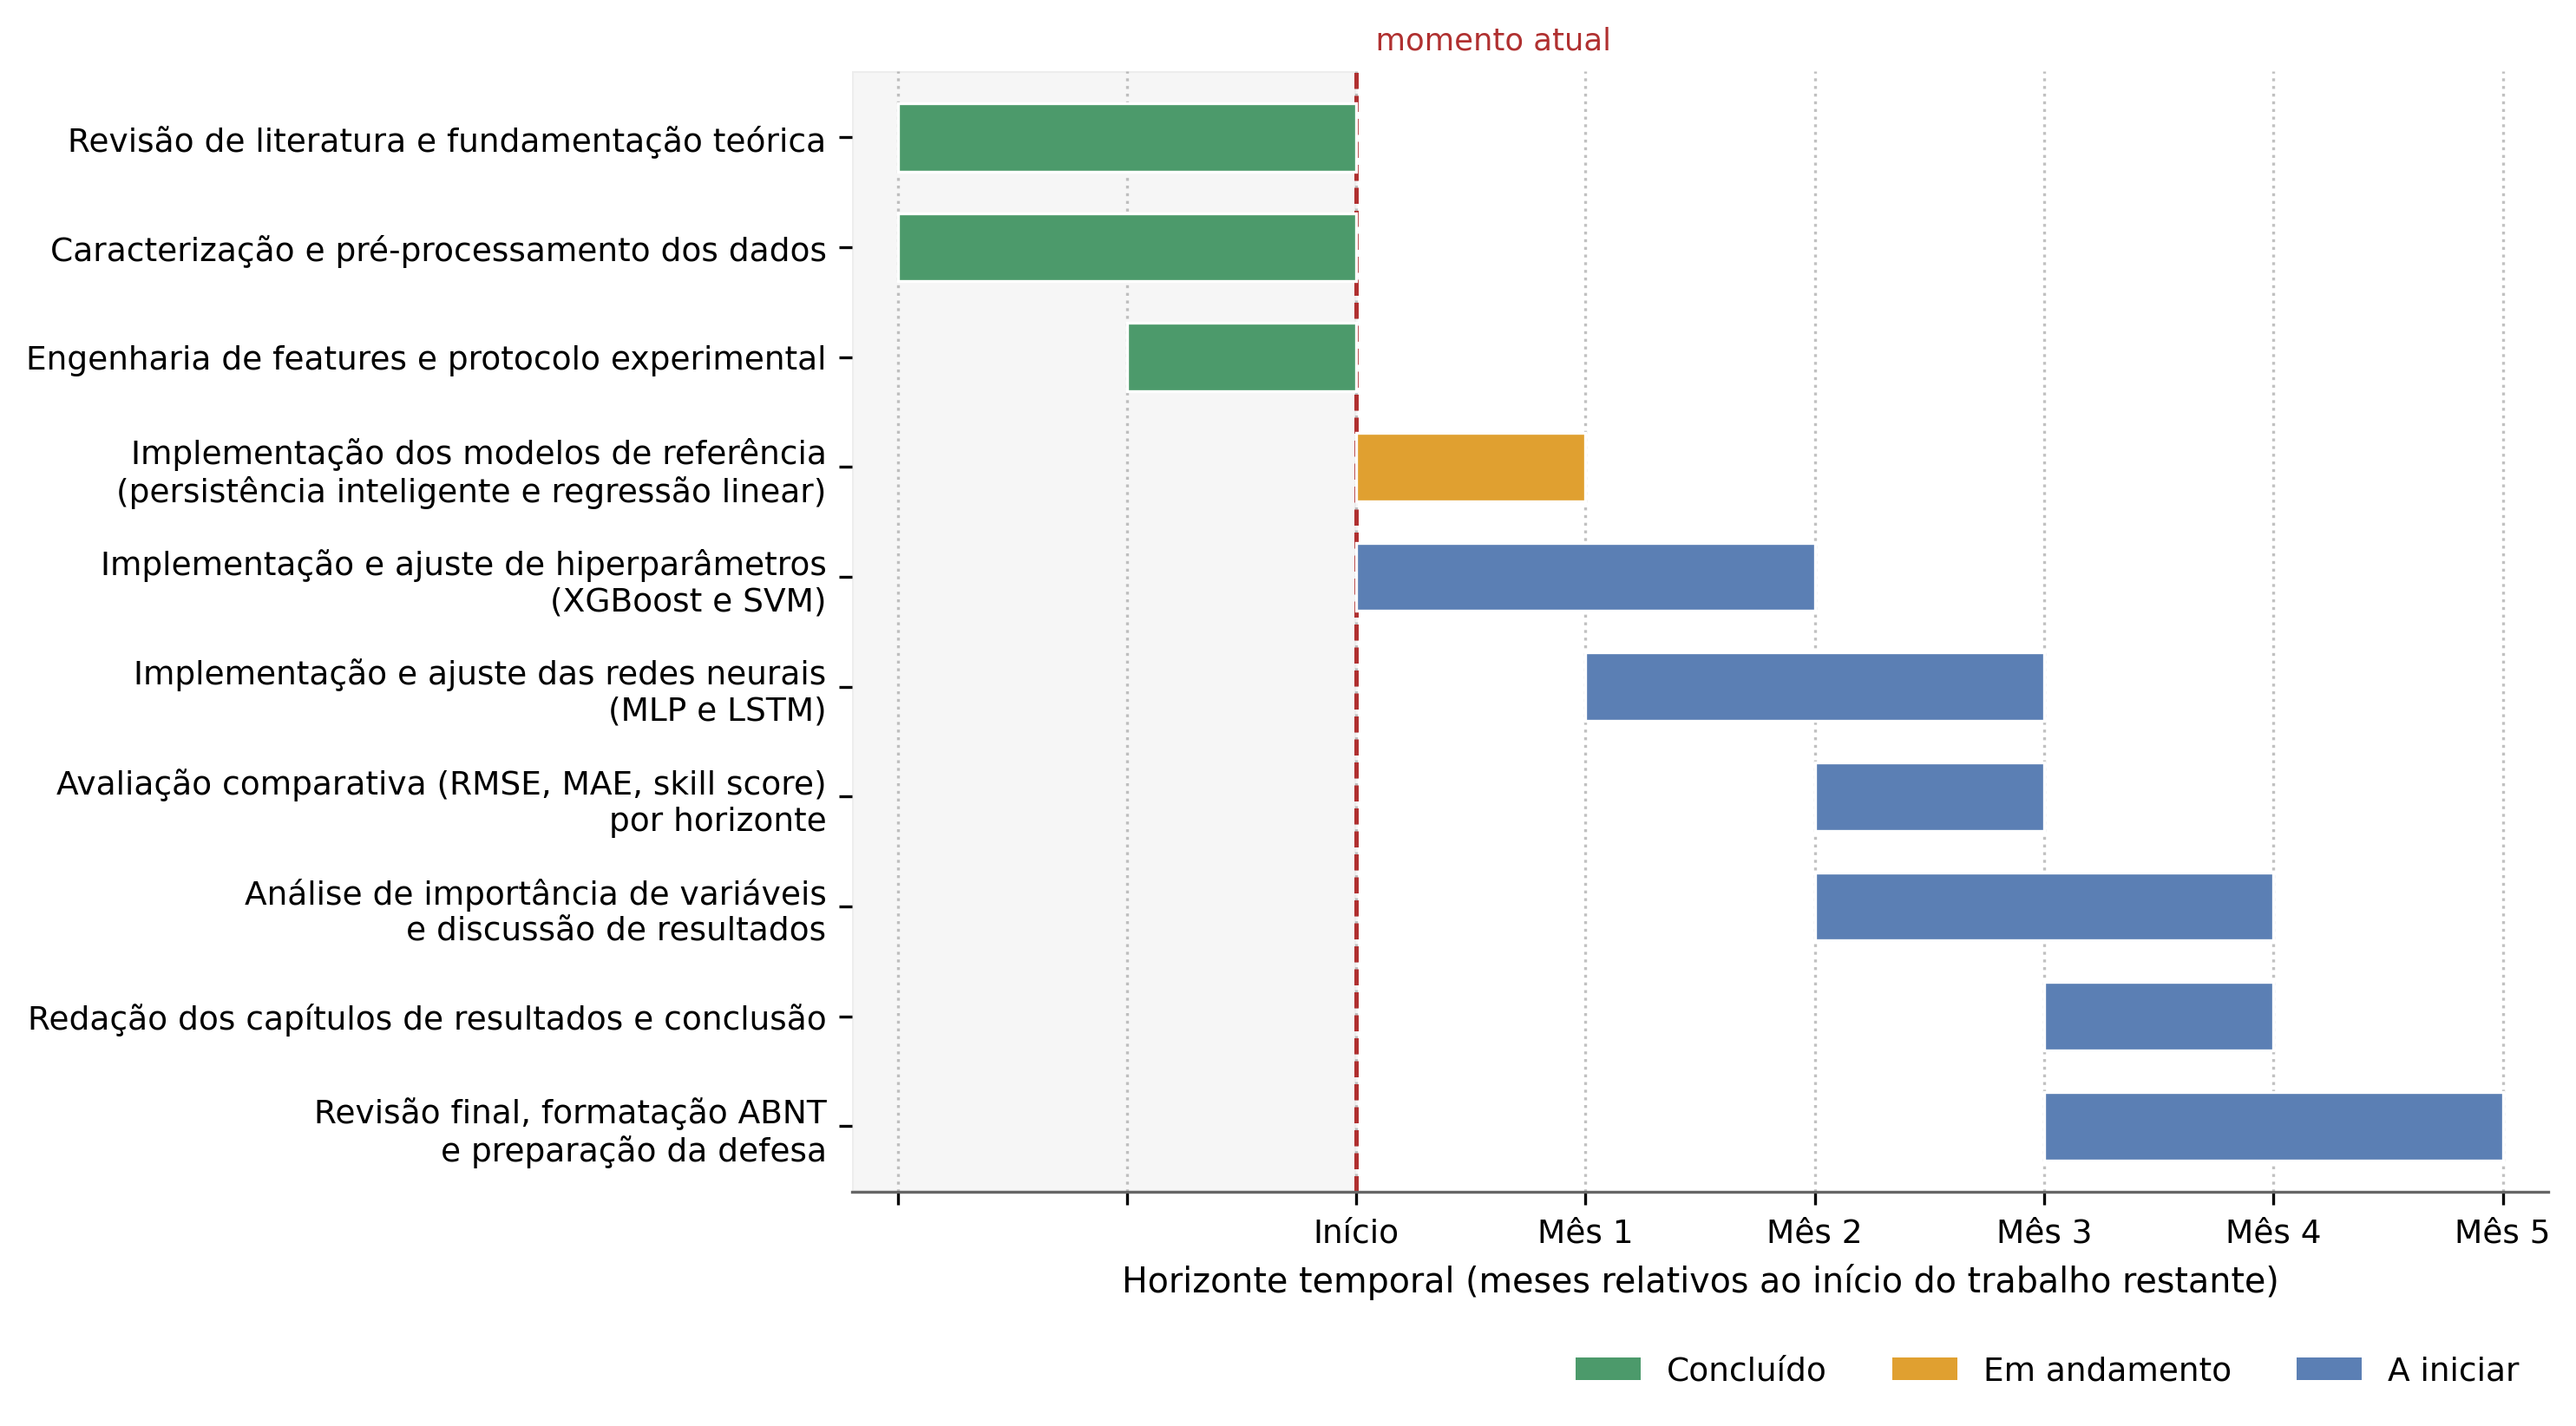
\includegraphics[width=\linewidth]{Images/gantt_cronograma.png}
\caption{Gráfico de Gantt das etapas restantes do trabalho. As barras em verde indicam atividades já concluídas; em âmbar, a etapa em andamento; em azul, as etapas a iniciar.}
\label{fig:gantt}
\end{figure}

\subsection{Riscos e pontos de atenção}

Três pontos merecem acompanhamento, antecipando questionamentos da banca: a \textbf{cobertura temporal limitada} (cerca de seis meses), que não abrange um ciclo sazonal completo e cujas implicações sobre a generalização serão discutidas explicitamente; o \textbf{desempenho esperado da LSTM}, que tende a ser superada por métodos baseados em árvores em regimes de poucos dados \citep{tian2023} — resultado de interesse sobre a adequação de cada classe ao regime de plantas em início de operação; e a \textbf{resolução do acordo de confidencialidade} com o operador, necessária antes da identificação do município e do estado na versão final.